%%%%%%%%%%%%%%%%%%%%%%%%%%%%%%%%%%%%%%%%%
% Beamer Presentation
% LaTeX Template
% Version 1.0 (10/11/12)
%
% This template has been downloaded from:
% http://www.LaTeXTemplates.com
%
% License:
% CC BY-NC-SA 3.0 (http://creativecommons.org/licenses/by-nc-sa/3.0/)
%
%%%%%%%%%%%%%%%%%%%%%%%%%%%%%%%%%%%%%%%%%

%----------------------------------------------------------------------------------------
%	PACKAGES AND THEMES
%----------------------------------------------------------------------------------------

%\documentclass{beamer}
\documentclass[12pt]{beamer}
\usepackage{keynote-portfolio}

\mode<presentation> {

% The Beamer class comes with a number of default slide themes
% which change the colors and layouts of slides. Below this is a list
% of all the themes, uncomment each in turn to see what they look like.

%\usetheme{default}
%\usetheme{AnnArbor}
%\usetheme{Antibes}
%\usetheme{Bergen}
%\usetheme{Berkeley}
%\usetheme{Berlin}
%\usetheme{Boadilla}
%\usetheme{CambridgeUS}
%\usetheme{Copenhagen}
%\usetheme{Darmstadt}
%\usetheme{Dresden}
%\usetheme{Frankfurt}
%\usetheme{Goettingen}
%\usetheme{Hannover}
%\usetheme{Ilmenau}
%\usetheme{JuanLesPins}
%\usetheme{Luebeck}
%\usetheme{Madrid}
%\usetheme{Malmoe}
%\usetheme{Marburg}
%\usetheme{Montpellier}
%\usetheme{PaloAlto}
%\usetheme{Pittsburgh}
%\usetheme{Rochester}
%\usetheme{Singapore}
%\usetheme{Szeged}
%\usetheme{Warsaw}

% As well as themes, the Beamer class has a number of color themes
% for any slide theme. Uncomment each of these in turn to see how it
% changes the colors of your current slide theme.

%\usecolortheme{albatross}
%\usecolortheme{beaver}
%\usecolortheme{beetle}
%\usecolortheme{crane}
%\usecolortheme{dolphin}
%\usecolortheme{dove}
%\usecolortheme{fly}
%\usecolortheme{lily}
%\usecolortheme{orchid}
%\usecolortheme{rose}
%\usecolortheme{seagull}
%\usecolortheme{seahorse}
%\usecolortheme{whale}
%\usecolortheme{wolverine}

%\setbeamertemplate{footline} % To remove the footer line in all slides uncomment this line
%\setbeamertemplate{footline}[page number] % To replace the footer line in all slides with a simple slide count uncomment this line

%\setbeamertemplate{navigation symbols}{} % To remove the navigation symbols from the bottom of all slides uncomment this line
}

\usepackage{graphicx} % Allows including images
\usepackage{booktabs} % Allows the use of \toprule, \midrule and \bottomrule in tables

%----------------------------------------------------------------------------------------
%	TITLE PAGE
%----------------------------------------------------------------------------------------

\title[NEUCOGAR]{NEUCOGAR} % The short title appears at the bottom of every slide, the full title is only on the title page

\author{Max Talanov} % Your name
\institute[IR ITIS KFU] % Your institution as it will appear on the bottom of every slide, may be shorthand to save space
{
IR ITIS KFU \\ % Your institution for the title page
\medskip
\textit{max.talanov@gmail.com} % Your email address
}
\date{\today} % Date, can be changed to a custom date

\begin{document}

\begin{frame}
\titlepage % Print the title page as the first slide
\end{frame}


%----------------------------------------------------------------------------------------
%	PRESENTATION SLIDES
%----------------------------------------------------------------------------------------

%------------------------------------------------
\section{The problem} % Sections can be created in order to organize your presentation into discrete blocks, all sections and subsections are automatically printed in the table of contents as an overview of the talk
%------------------------------------------------
%------------------------------------------------

\begin{frame}
\frametitle{What is the main problem?}
\begin{columns}[c] % The "c" option specifies centered vertical alignment while the "t" option is used for top vertical alignment

\column{.45\textwidth} % Left column and width
\begin{enumerate}
\item Why do we need conscious machines?
\item What is consciousness?
\item What is intelligence?
\end{enumerate}

\column{.6\textwidth} % Right column and width
%------------------------------------------------
\begin{figure}
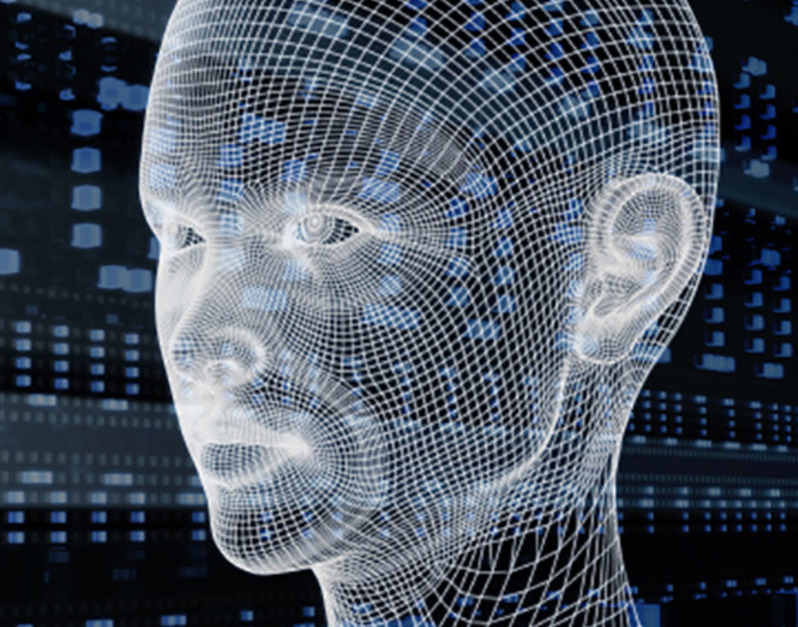
\includegraphics[width=1.0\linewidth]{AI_1}
\end{figure}
%------------------------------------------------
\end{columns}
\end{frame}

%------------------------------------------------

\begin{frame}
\frametitle{Consciousness $\rightarrow$ Emotions}
\begin{columns}[c] % The "c" option specifies centered vertical alignment while the "t" option is used for top vertical alignment

\column{.45\textwidth} % Left column and width
\textbf{Human:}
\begin{itemize}
\item Cognition $\Rightarrow$ Consciousness $\Rightarrow$ Emotions
\end{itemize}

\textbf{Machine:}
\begin{itemize}
\item Cognition $\Rightarrow$ Consciousness $\Rightarrow$ Emotions
\end{itemize}

\column{.6\textwidth} % Right column and width
%------------------------------------------------
\begin{figure}
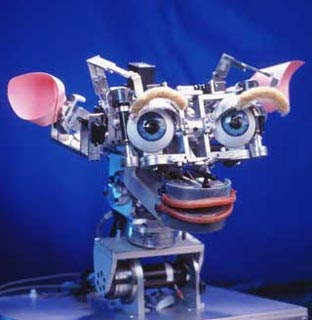
\includegraphics[width=1.0\linewidth]{Kismet_312}
\end{figure}
%------------------------------------------------
\end{columns}
\end{frame}

%------------------------------------------------

\begin{frame}
\frametitle{Robot emotions}
\begin{columns}[c] % The "c" option specifies centered vertical alignment while the "t" option is used for top vertical alignment

\column{.3\textwidth} % Left column and width
\begin{enumerate}
\item Why do mammals need emotions?
\item Why do robots need emotions?
\end{enumerate}

\column{.3\textwidth} % Right column and width
%------------------------------------------------
\begin{figure}
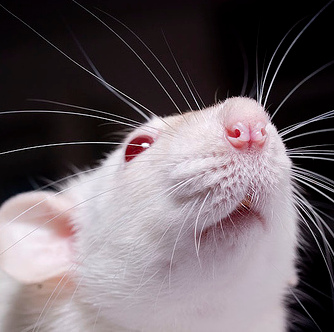
\includegraphics[width=1.0\linewidth]{rat}
\end{figure}
%------------------------------------------------

\column{.3\textwidth} % Right column and width
%------------------------------------------------
\begin{figure}
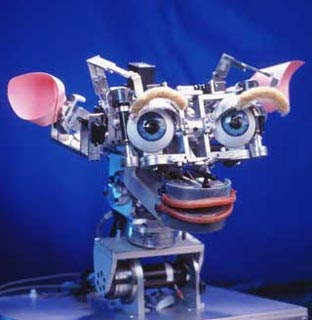
\includegraphics[width=1.0\linewidth]{Kismet_312}
\end{figure}
%------------------------------------------------
\end{columns}
\end{frame}

%------------------------------------------------
\section{Cube of emotions}
%------------------------------------------------

\begin{frame}
\frametitle{Cube of emotions}
\begin{figure}
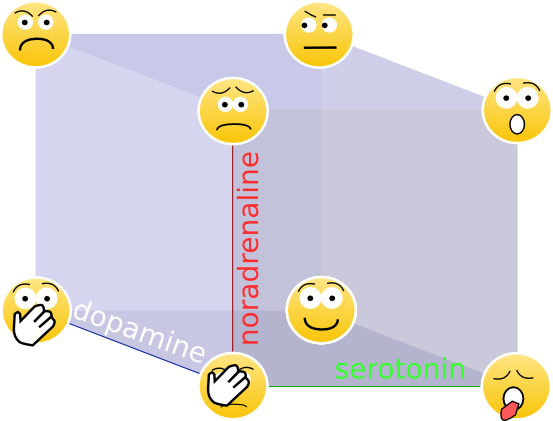
\includegraphics[width=0.9\linewidth]{cube_of_emotional_parameters}
\end{figure}
\end{frame}

%------------------------------------------------

%------------------------------------------------

\begin{frame}
\frametitle{Machine emotions}
\begin{figure}
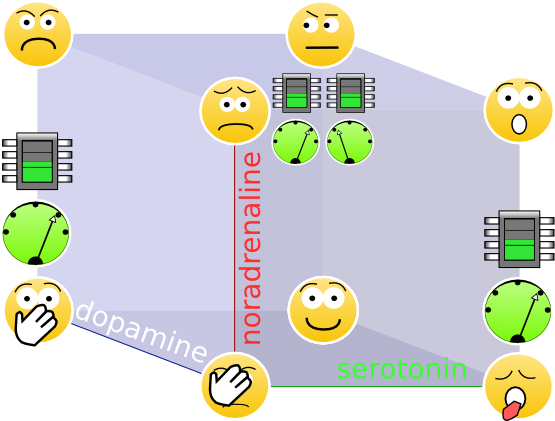
\includegraphics[width=0.9\linewidth]{cube_of_emotional_parameters_machine}
\end{figure}
\end{frame}

%------------------------------------------------

%------------------------------------------------

\begin{frame}
\frametitle{Experiment}
\begin{figure}
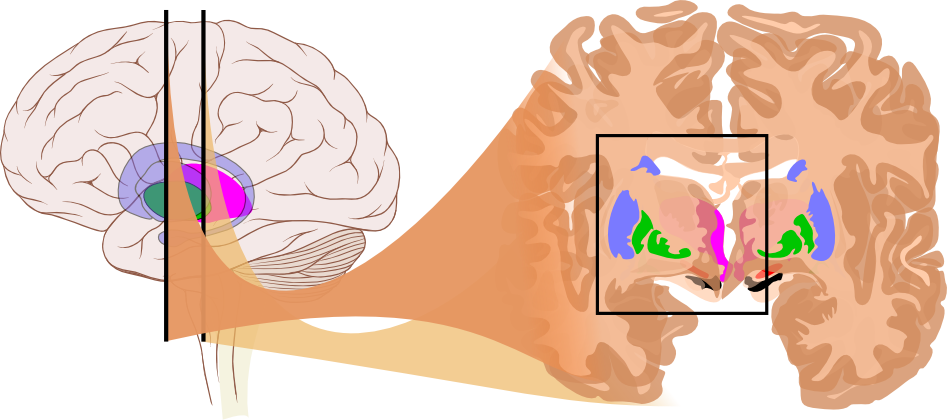
\includegraphics[width=1.0\linewidth]{Basal_ganglia_circuits_cropped}
\end{figure}
\end{frame}

%------------------------------------------------

%------------------------------------------------

\begin{frame}
\frametitle{Result}
\begin{figure}
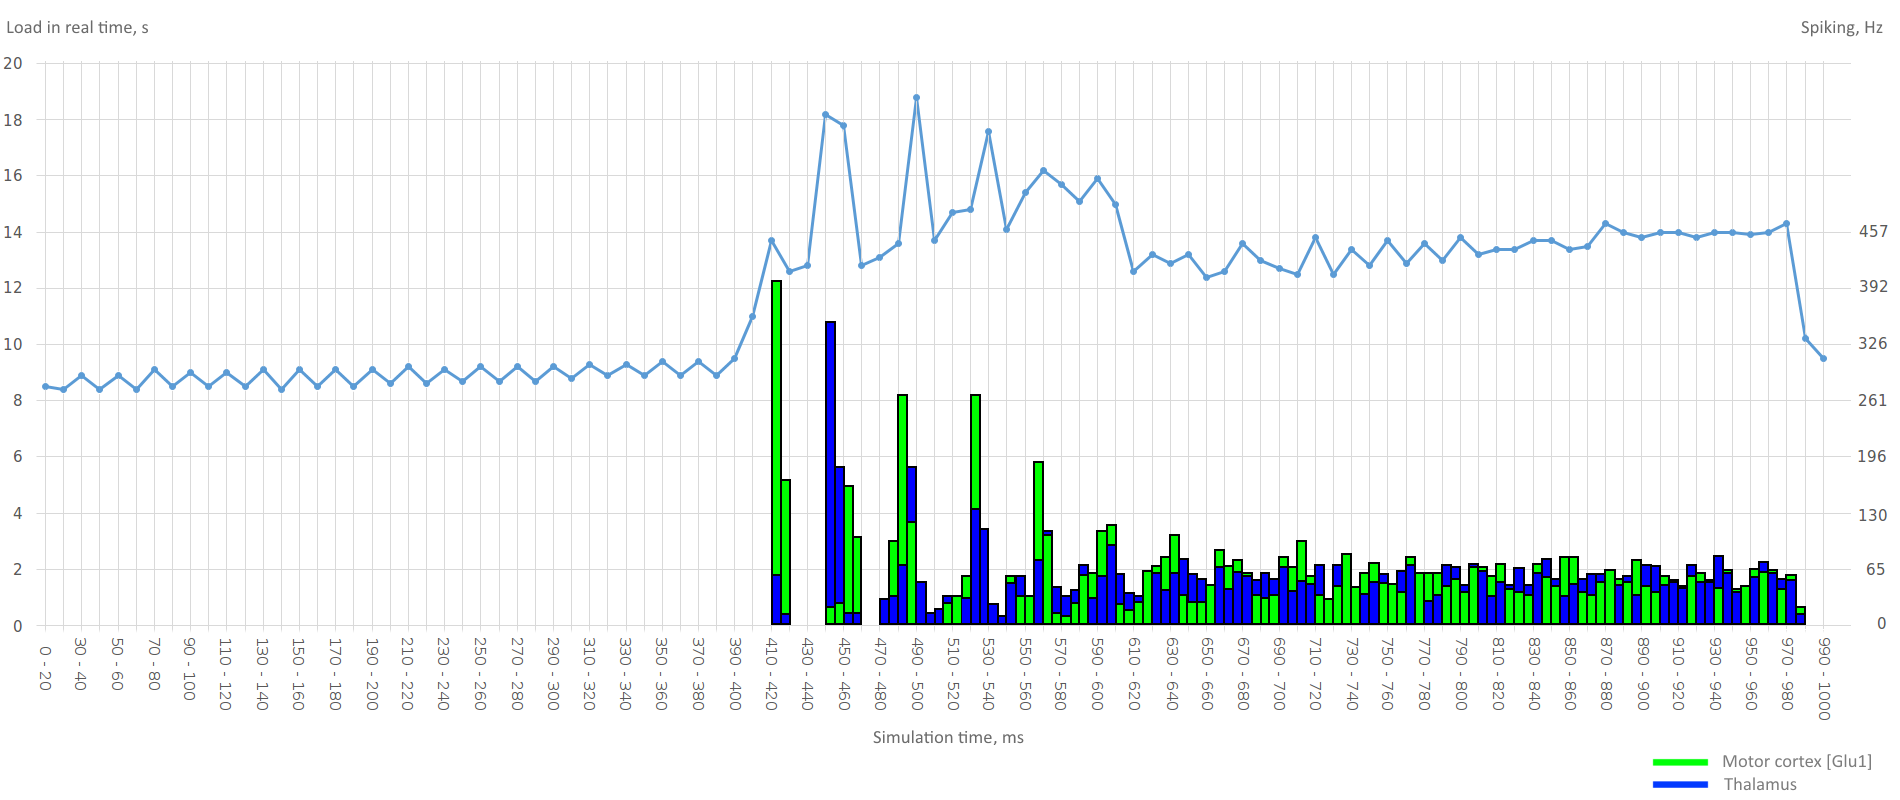
\includegraphics[width=1.0\textwidth]{resultBIG}
\end{figure}
\end{frame}

%------------------------------------------------
%------------------------------------------------

\begin{frame}
\frametitle{Thank you}
\begin{figure}
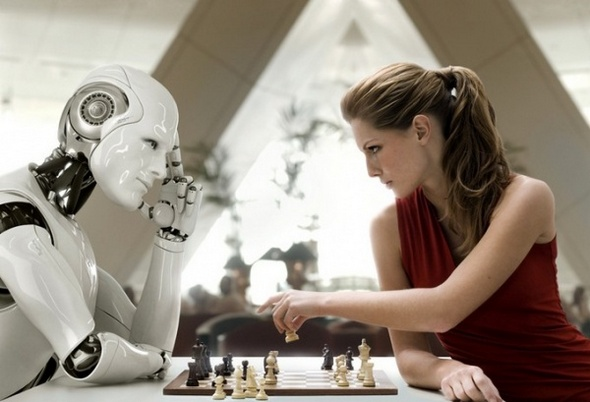
\includegraphics[width=0.8\linewidth]{ai_chess}
\end{figure}
\end{frame}

%------------------------------------------------

\end{document} 
